\documentclass[a4wide, 11pt]{article}
\usepackage{a4, fullpage}
\usepackage{graphicx}
\setlength{\parskip}{0.3cm}
\setlength{\parindent}{0cm}

% This is the preamble section where you can include extra packages etc.

\begin{document}

\title{Webapps Project 2014: Final Report}

\author{Alan Vey, Octavian Tuchila, Sean Naderi}

\date{June 11, 2014}         % inserts today's date

\maketitle            % generates the title from the data above
\clearpage

\section{Introduction}
\clearpage

\section{Project Management}
\subsection{Group Structure}
Alan was the group leader and in charge of the planning of the assignment. He also was the primary developer and so set up the project, wrote the code for all functionality of the site and sorted out all research into third party tools and deployment options. He also set up the testing infrastructure for the application.

In the beginning stages, Octavian was in charge of developing the file system to be used for the site but was met with several difficulties and so after looking into the problems, Alan realised that we could incorporate EtherPad for collaborative document editing, which handles storage itself. Thus, Octavian was assigned to the design of the entire website. 

Sean was put in charge of adding additional tests for new features and design elements. Sean used our project to plan our presentation. His feedback was useful in hashing out the small details of the site for both functionality and design.

\subsection{Implementation Language}
We decided to use the Ruby on Rails framework to develop our application. This meant between us we needed knowledge of Ruby, JavaScript/CoffeeScript, HTML and embedding, CSS and of course the Rails framework itself. Domain specific languages such as RSpec, Capybara and Factorygirl also played a role. Limited knowledge of SQL aided some debugging issues we had relating to the database.

All three of us worked on the WACC complier project together which we implemented in CoffeeScript and JavaScript giving us a solid foundation in these languages. The Ruby on Rails exercise had taught us the basics of web development so combined with the fact that none of us had any prior experience creating web based applications at least we has a good understanding of these languages. This was one of the main reasons for choosing Rails. 

We all found it really useful learning Haskell, Java and C when we first commenced our studies as these are all strongly typed languages and have a ridged development style which lead to a very solid understanding of programming. We wanted to apply the same principal to web applications by learning to develop with a framework that has a ridged set of development principals before using tools which allow for more freedom. 

Considering most of our programming knowledge is in the three languages mentioned above, we though expanding our understanding of dynamic ones would greatly benefit us making Ruby and JavaScript/CoffeeScript ideal. The process of embedding both in HTML and making use of the reflective nature of Ruby has been really interesting.

A start up Alan is working on in the summer makes use of this framework and so he was especially keen on finding out more about it. 

\subsection{Design Process}
Our division of labour lead to an efficient design process. There was no code duplication and since our responsibilities allowed for little overlap we did not have to spend much time combining the different elements. 

Initially, Alan considered using pivotal tracker to plan out our project, however this seemed to offer more functionality than required and would lead to too much complexity in setting up the project so we settled on Git, Gitlab milestones/issues and our website itself. Communication was taken care of by having regular meetings planned by Alan as well as a Facebook group chat and FaceTime. 

We used Git as a backup and collaborative development tool. Alan set up the project and got a solid foundation implemented, tested and pushed to our master branch. 
From this point onwards any new functionality Alan added was done on a separate branch and merged in upon completion. 
Octavian would branch every time new functionality was added to manage the design of that part of the newly added components and merge with master when he was done. 
Sean would await the completion of functionality at which point he branched off and conducted modular testing of the models, merging back in when done and branch off again when the design was done to conduct integration testing again merging his work back to master upon completion. 

At the beginning of the project we thought of the milestones that were required and set them up on Gitlab [Figure~\ref{fig:Github}]. We subsequently added issues when they arose or we started working on a new section, assigning them to whoever we felt was best equipped to deal with them and allocating them to a milestone. This was very useful to know exactly who was working on what and making sure any problems a team member discovered were addressed by the appropriate party. 

During the feedback for our Milestone 1 review, Mark suggested we use our site to plan a part of this project. We really liked the idea and decided to plan the presentation with it writing up all supporting documentation on our collaborative real-time software. This was not only useful for the organisation of the presentation but allowed us to find minor bugs and improvements for our site. 

We usually met every two to three days to make sure the project was on track and do any of the additional tasks as well as help each other out with what we had learned. Sean would record meeting minutes and send everyone a copy on our Facebook group if required. Octavian took a keen interest in the legal aspects and helped Sean and Alan gain a better understanding after some research he had conducted. The meetings were planned using a Facebook group chat which also served as a useful tool for sharing links we found important and helping each other out with any issues we came across that we did not need to meet for.

All in all we feel this project has been a success as we have overcome many difficulties we encountered in previous tasks we completed together such as code duplication, missing deadlines, under performing and not helping each other adequately. We will definitely be planning future tasks in much more detail as we have done with this one and have all learned a lot about all the software we used to facilitate this.

\begin{figure}
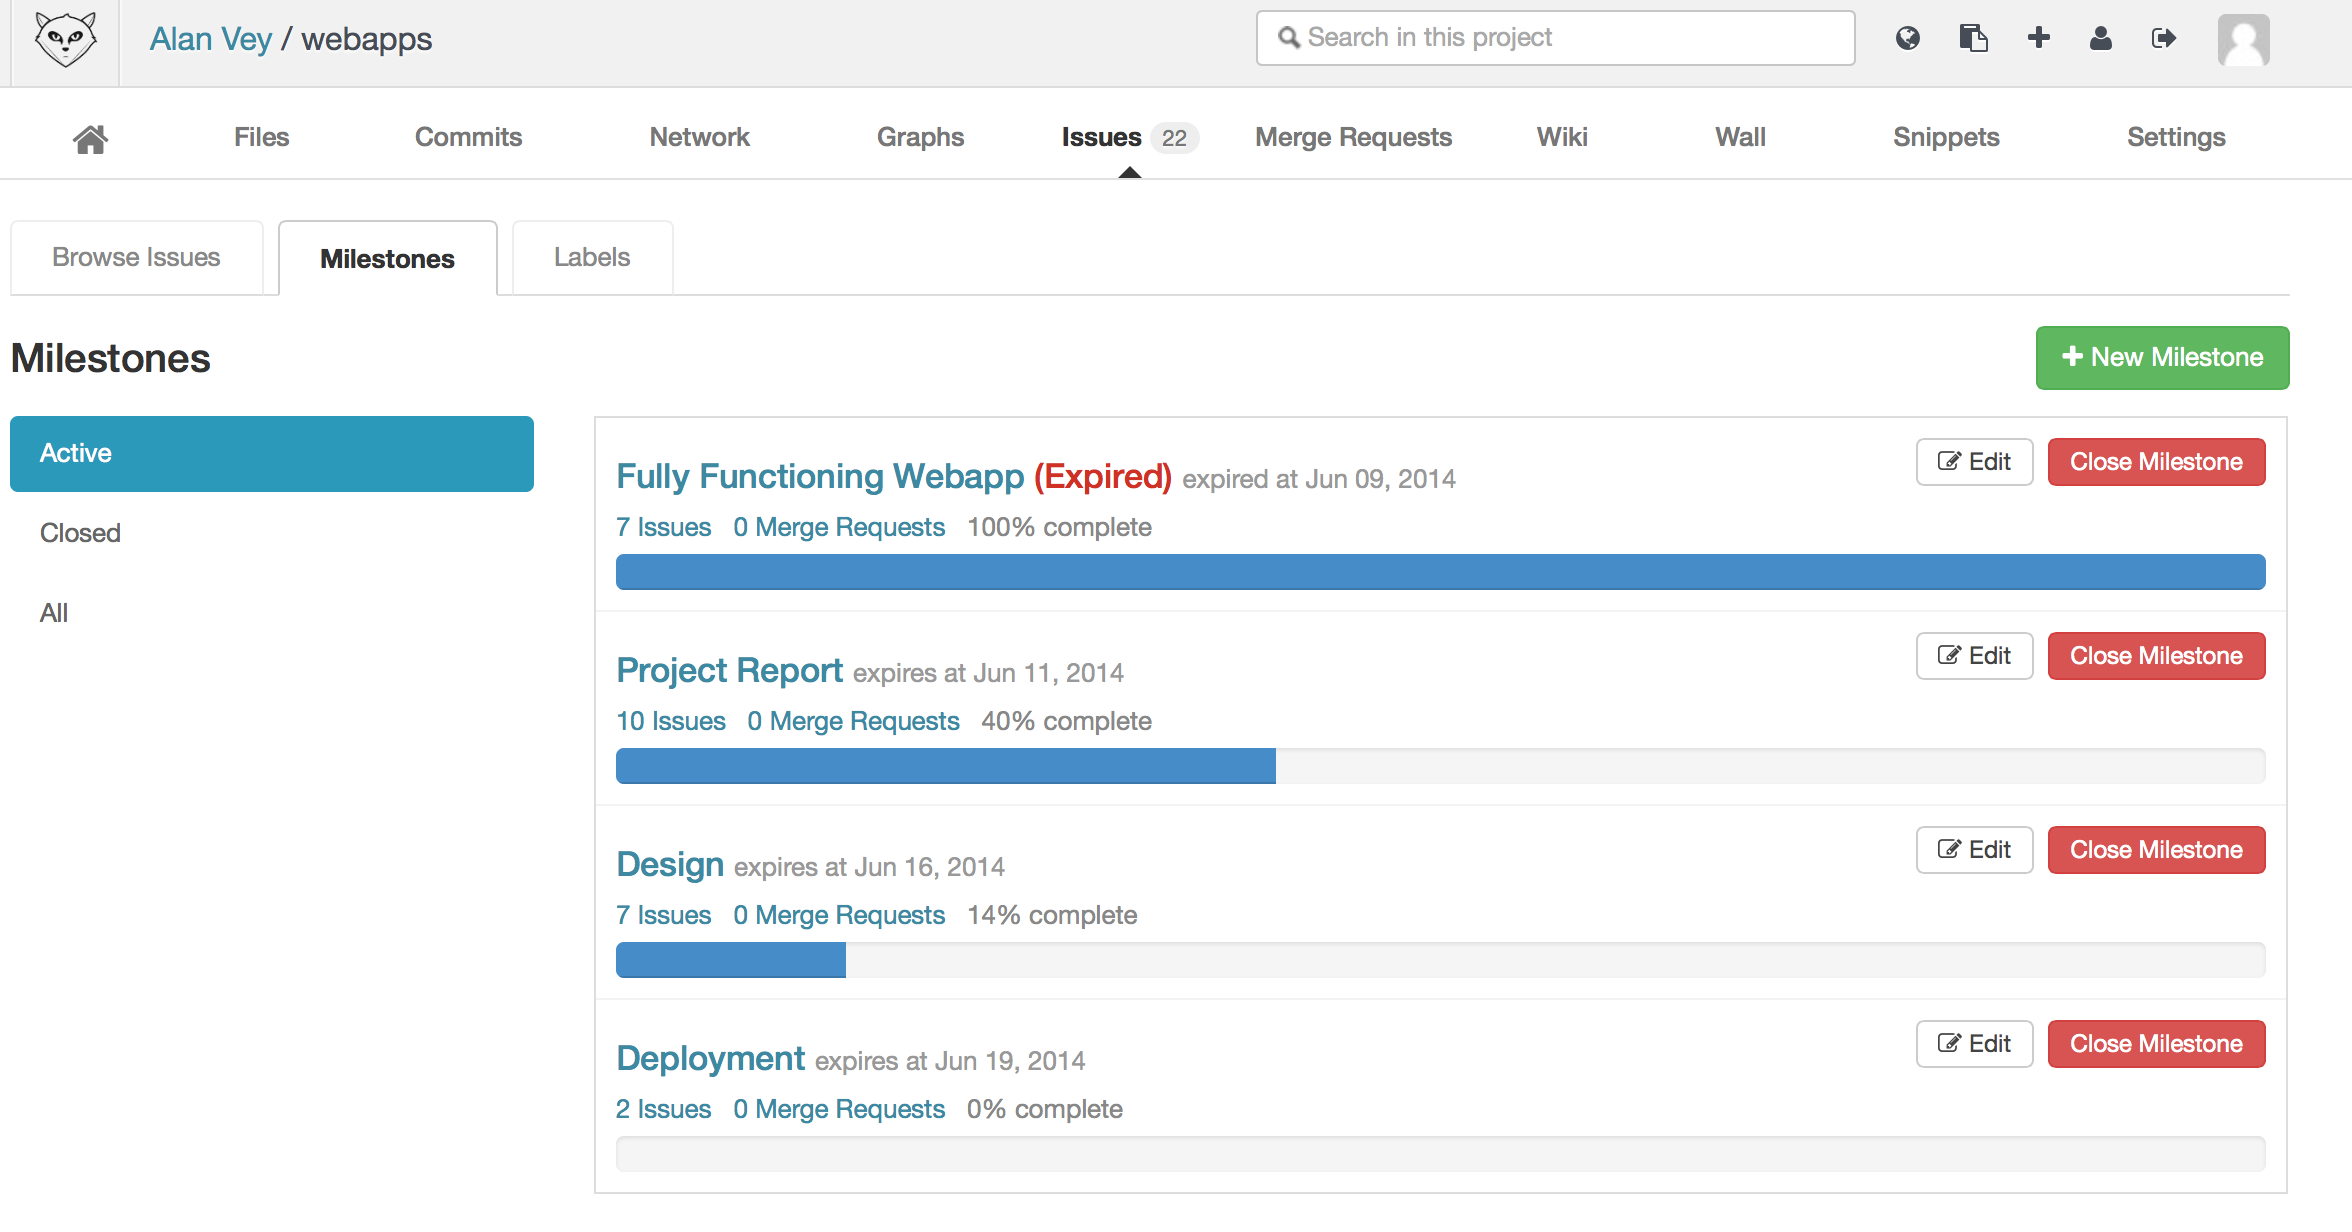
\includegraphics[width=1\textwidth]{gitlab-milestones.png}
\caption{Overview of milestones on June 10, 2014}
\label{fig:Github}
\end{figure}

\clearpage

\section{Program Description}
\subsection{Some Code} 

\begin{verbatim}
    The verbatim environment outputs the source without changing
    it in any way. 
          This
              includes line breaks
       and indentation. 
    It is useful to reproduce code snippets.
\end{verbatim}
\clearpage

\section{Legal Aspects}

We've used the Ruby programming language, together with several ruby gems.
These are under the Ruby Licence, which has been accepted by the Free Software
Foundation as compatible under the GPL(General Public Licence)\cite{GNUlicence}
but has not been accepted by the Open Source Initiative. The Ruby Licence has a
copyleft status, which allows copying the code, as long as the application
which is built using Ruby Licenced software is bound by the same licence. The
Ruby software has a dual licence, both under the Ruby Licence and under the
simplified BSD licence.

If we want to publish our project, we can do so under the Ruby Licence.
In order to do this, we have the following options:

\begin{quote}
3. You may distribute the software in object code or binary form,
   provided that you do at least ONE of the following:

a) distribute the binaries and library files of the software,
together with instructions (in the manual page or equivalent)
on where to get the original distribution.

b) accompany the distribution with the machine-readable source of
the software.

c) give non-standard binaries non-standard names, with
instructions on where to get the original software distribution.

d) make other distribution arrangements with the author.
     \cite{Rubylicence}
\end{quote}

In case we want to use the website commercially, we should act on clause
d, by contacting the author of the Ruby programming language and the authors of
the gems we have used while building our project.

Another option for commercial distribution is to use JRuby instead of the Ruby
interpretor, as it can support Rails projects and its licence is more suitable
for commercial releases.

\begin{quote}
this license is intended to facilitate the commercial use of the Program
\cite{JRubylicence}
\end{quote}

We can launch our project using the following clause:

\begin{quote}
a) Subject to the terms of this Agreement, each Contributor hereby grants
Recipient a non-exclusive, worldwide, royalty-free copyright license to
reproduce, prepare derivative works of, publicly display, publicly perform,
distribute and sublicense the Contribution of such Contributor, if any, and
such derivative works, in source code and object code form.
\cite{JRubylicence}
\end{quote}
\clearpage

\section{Conclusion}

\subsection{Our project}
We have managed to successfully design a fully functional project management and real-time collaborative editing tool. We have user authentication, the functionality for project creation and a  split of every project into the categories of overview, management and editing. 

When navigating to our site one lands on the home page and can access no more until authenticated. Upon successful login the home page is no longer accessible and by default the root is set to a page listing all projects one has created or is a team member of. Clicking on any project name leads to the show page and results in a new navbar with the three categories for project design.

As the name suggests, overview gives a brief summary including the project name, description, owners email, team members and a Burndown chart to visually illustrate the progress. There is a two tier hierarchy where the project creator can edit the name and description and add team members however all other functionality is the same for any user. Obviously a project can only be accessed by the creator or a team member. 

The management page, accessible from the secondary navbar, displays a listing of milestones. Once created one can navigate to a show page for the milestone which allows for the creation of tasks and has a news feed of the most recent comments on all already created tasks. Each task can be commented on manually by navigating to their respective show pages or automatically by clicking on start and then finish and then reviewed. Again a hierarchy is used here so that only the person who started the task can finish it and only the creator of the task can review it.

The edit page contains a listing of file names and allows for the creation of additional ones. Once created, clicking on a file navigates to its respective show page which loads up the file in editing software and allows any team member working on the file to do so simultaneously, all of which is visible to ever user on the page in real-time. This software incorporates chat functionality as well as the optional download of the file. 

\subsection{Possibilities for improvement}
There are very many things we would have liked to add to our website, the main five being:
\begin{itemize}
  \item Help and supporting documentation
  \item User profiles and Private messaging
  \item Email notifications
  \item Contribution analysis
  \item Real time collaborative software for spreadsheets and presentations
  \item Gitlab integration
\end{itemize}

Supporting documentation, interactive explanations and help on the site is the most important thing missing as far as we can tell. For example whenever creating anything a small question mark would exist next to the label for the any field, which when hovered over would explain exactly what the field means and if one clicked on details would describe how it affects the project. For example creating a task; Hovering over the question mark for the difficulty would explain that this is used to keep the project on track and plays a role in the dynamic creation of the chart on the overview page. Details would redirect to the help page in a new tab, and would go into detail of the Burndown chart algorithms used.

User profiles is also a key element for improvement. Tracking the quality of users contribution as well as having some sort of team mate rating scheme and number of projects worked on would build up useful data about users which could then be used as a sort of resume when applying to work on certain projects or allow project creators to find team members with the desired skill sets. This would be modelled after websites like LinkedIn.

Email notifications are also very necessary, whether its providing updates of whats happening on projects one is part of, notification of received private messages or later notifying users of potential project prospects or suggesting team members to creators.
 
\subsection{Learning aspects}
Because Rails incorporates the basics of CSS/CSSASS, HTML and embedding, JavaScript/CoffeeScript and obviously Ruby, using the framework provided us with a substantial understanding of these tools and how to incorporate them into the framework itself. 

Furthermore, since Rails heavily relies on test driven development, and since RSpec was included, behaviour driven development and the MVC pattern we gained experience and knowledge regarding the application of the principles we learned in the software engineering module. Our understanding of the principals of cohesion and coupling were also improved in the creation of the interactive charting class.

Besides the computing aspects we have all learned a significant amount about project management, considering the amount of research that went into creating this site. Working on this project whilst applying the learned concepts, in an attempt to provide the simplest most efficient experience possible for our users, really highlighted any mistakes we had been making and allowed us to further improve the site.
\clearpage

\subsection{Difficulties}
The main possibility for improvement would be for all of the team to learn the framework in a lot more depth at the beginning of the project. This would have allowed every team member to contribute towards the functionality of the site and thus a shorter list of unimplemented features. It would also have allowed for team members to review and improve each others work more and so arrive at a more robust and efficient end product.

Another aspect is planning. We started this project in what we thought was an organised manner, however based on what we have learned now highlights the fact that this was not quite the case. The use of planning software leads to much higher productivity and would also have lead to a shorter list of unfitted functionality. 

We have worked on many projects together so had already addressed many issues like organisation leading to code duplication and inefficiency in the past. All in all we feel this project has been a great success and we have all taken away a lot from it.

\begin{thebibliography}{9}

\bibitem{GNUlicence}
  http://www.gnu.org/philosophy/license-list.html\#Ruby

\bibitem{Rubylicence}
  https://www.ruby-lang.org/en/about/license.txt

\bibitem{JRubylicence}
  https://github.com/jruby/jruby/blob/master/COPYING
\end{thebibliography}

\end{document}
